\chapter{Testen der Hyperparameter in DSEA und neuronalen Netzen}
In diesem Kapitel werden die Ergebnisse präsentiert und diskutiert.
Vorerst wird der verwendete Datensatz charakterisiert und die Schritte der Daten-Vorverarbeitung beschrieben.
In \autoref{sec:nn_no_dsea} wird die Entfaltung über eine Klassifikation mit einem NN analysiert.
Ebenfalls wird bereits das Spektrum über die Aufsummierung der Konfidenzen rekonstruiert.
Hinzu kommt die iterative Anpassung der Gewichte, in \autoref{sec:deconv_dsea}.
Es werden neuronale Netze in DSEA systematisch über eine Gittersuche analysiert.
Anschließend wird der Trainingsprozess, die entfalteten Spektren und Korrelationen betrachtet.
Zum Schluss, wird in \autoref{sec:bias} die Abhängigkeit der Modelle vom Trainingsspektrum untersucht.

\section{Datensatz}
Der Monte-Carlo Datensatz 11374 \cite{dataset} beinhaltet Neutrinos mit einem simulierten Spektrum $E^{-2}$.
Es werden nur sog. "`upgoing"'  Neutrinos betrachtet.
Das sind Neutrinos die vor der Detektion die Erde durchquert haben.
Es wurde bereits eine Eventauswahl durchgeführt.
\begin{table}
    \centering
    \caption{Statistische Kennzahlen zu der Energie des primären Neutrinos.
    Links für die ursprünglichen MC-Daten (Rohdaten) und im direkten Vergleich, der abgeschnittene Datensatz mit Energien $\leq \SI{100}{\tera\eV}$ (rechts).
    }
    \label{tab:energy_stats}
    \begin{tabular}{l|c c}
        \toprule
        & Rohdaten & Daten nach Schnitt \\
        \midrule
        Anzahl Events & $\SI{1.334e+7}{}$ & $\SI{1.326e+7}{}$\\
        Mittlere Energie $\mu$ & $\SI{6.3}{\tera\eV}$ & $\SI{2.2}{\tera\eV}$ \\
        Standardabweichung $\sigma$ & $\SI{246}{\tera\eV}$ & $\SI{7}{\tera\eV}$ \\
        Minimum & $\SI{100}{\giga\eV}$ & $\SI{100}{\giga\eV}$ \\
        Maximum & $\SI{e+8}{\giga\eV}$ & $\SI{e+5}{\giga\eV}$ \\
        $\SI{25}{\percent}$-Quantil & $\SI{271}{\giga\eV}$ & $\SI{270}{\giga\eV}$ \\ 
        $\SI{50}{\percent}$-Quantil & $\SI{547}{\giga\eV}$ & $\SI{543}{\giga\eV}$ \\ 
        $\SI{75}{\percent}$-Quantil & $\SI{1.42}{\tera\eV}$ & $\SI{1.39}{\tera\eV}$ \\ 
        \bottomrule
    \end{tabular}
\end{table}
Dazu wird der Zenitwinkel mit einem Fehler von \SI{5}{\degree} rekonstruiert und Events von \SIrange{86}{180}{\degree} beibehalten.
Dies hat den Vorteil, dass keine Signaturen von Myonen beachtet werden müssen.
Die Myonen wechselwirken mit der Erde und können den Detektor nicht erreichen.
Anders als für Myonen, stellt die Erde für Neutrinos kein Hindernis dar.
Aufgrund des geringen Wirkungsquerschnitts erreichen die meisten Neutrinos den Detektor.
Der Datensatz beinhaltet 13 Millionen Events.
Die Energie des primären Neutrinos stellt die Zielvariable des Klassifikationsproblems dar.
In \autoref{tab:energy_stats} sind wichtige Informationen über die Lage und Streuung der Neutrinoenergie aufgeführt.
%%%%%%%
Auffällig ist, dass der größte Teil der Events im niederenergetischem Bereich liegt.
Augrund der geringen Statistik im Hochenergiebereich werden nur Events unter $\SI{100}{\tera\eV}$ berücksichtigt.
Die untere Energiegrenze bleibt unverändert und beträgt $\SI{100}{\giga\eV}$.
Mit einer logarithmischen Skala wird die Energie in 10 Klassen aufgeteilt.
Das logarithmische Binning kompensiert zum Teil die wenigen Events im Hochenergiebereich.
Wird mit realen Daten gearbeitet, so können an dieser Stelle Under- und Overflow-Bins eingeführt werden.
Diese decken den für die Analyse nicht-relevanten Bereich ab.
$\SI{90}{\percent}$ der Events werden zum Trainieren und die restlichen Events zur Evaluation des Modells verwendet.
\\
Die 12 Features (siehe \autoref{tab:feature}) werden vor der Entfaltung normalisiert
\begin{equation*}
    z = \frac{x-\mu}{\sigma}
\end{equation*}
um gleiche Abstände zwischen den Features zu gewährleisten.
Dies ist ein notwendiger Schritt zur Optimierung des Trainingsprozesses \cite{scaler}.

% NN OHNE DSEA
\section{Entfaltung als Klassifikationsproblem} \label{sec:nn_no_dsea}
Die Betrachtung der Entfaltung als Klassifikationsproblem ist eine der grundlegenden Ideen von DSEA.
In diesem Kapitel soll vorerst die Entfaltung über eine klassische Klassifikation diskutiert werden.
Die \autoref{fig:single_event} zeigt exemplarisch die Vorhersage eines einzelnen Events.
Die Zugehörigkeit des Events zum $j$-ten Energie-Bin wird durch die Konfidenz $c_j$ angegeben.
Ein Datenpunkt wird nach dem Prinzip \textit{maximum a posterioro} der Klasse mit der \textbf{maximalen Konfidenz} zugeordnet \cite{max_pred}:
\begin{equation*}
    \hat{y} = \underset{j}{\arg\max} \{ c_j \}, \qquad j=[0,...,n-1]
\end{equation*}
Die Anzahl der Energie-Bins ist über $n$ definiert.
Das NN wird auf den Trainingsdaten mit \SI{50}{\text{Epochen}} trainiert.
In \autoref{tab:nn_params} sind die verwendeten Hyperparameter des NN aufgeführt.
\SI{500000}{\text{Events}} der Evaluationsdaten werden entfaltet und analysiert.
Ein Event wird jeweils der maximal vorhergesagten Klasse zugeordnet.
Die Kostenfunktion, sowie die Metriken werden in jeder Epoche im Trainingsprozess für die Trainings- und Evaluationsdaten ausgewertet.
Der Verlauf der kategorischen Kreuzentropie und der $\Chi^2$-Distanz ist in \autoref{fig:NN_history} dargestellt.
\\
\begin{wrapfigure}{l}{.5\textwidth} %[17]{l}{.5\textwidth}
    \centering
    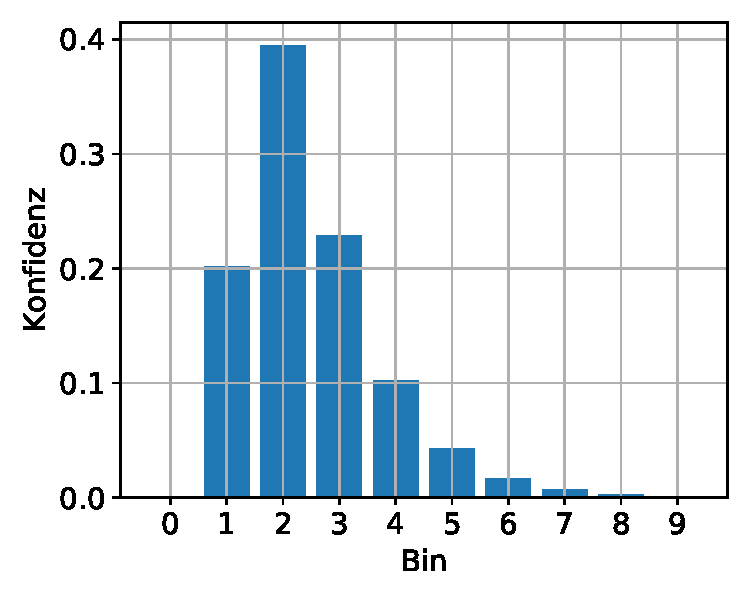
\includegraphics[width=.5\textwidth]{Plots/NN/single_events_class2.pdf}
    \caption[Graphische Darstellung der Ausgabe des NN]{Visuelle Darstellung der Ausgabe des NN für ein Event mit der wahren Energieklasse 2.
    Die Zugehörigkeit des Events zu Bin $j$ ist durch die Konfidenz $c_j$ definiert.
    }
    \label{fig:single_event}
\end{wrapfigure}
Die $\Chi^2$-Distanz, als Abstandsmaß zwischen dem wahren und vorhergesagten Spektrum konvergiert.
Ebenso verläuft der Verlust der Evaluationsdaten gegen ein Minimum.
Der Anstieg des Trainingsverlusts deutet auf ein leichtes Overtraining ("`Übertrainieren"') hin.
Eine Fortsetzung des Trainings ist daher nicht sinnvoll.
Das resultierende Spektrum in \autoref{fig:NN_spectrum_hard} weist starke Abweichungen von der wahren Verteilung auf.
Bins im hochenergetischen Bereich werden stark unterschätzt, hingegen werden die Bins bis etwa \SI{1}{\tera\eV} überschätzt.
Aufgrund der geringen Accuracy von $\sim\SI{39}{\percent}$ kommt es zu vielen Fehlklassifikationen.
Siehe dazu den Verlauf der Accuracy im Trainingsprozess \autoref{fig:NN_acc}.
Die Korrelation zu ähnlichen Energien bzw. benachbarten Bins wird hier nicht berücksichtigt.
\begin{figure}%
    \begin{subfigure}{0.5\textwidth}%
        \centering%
        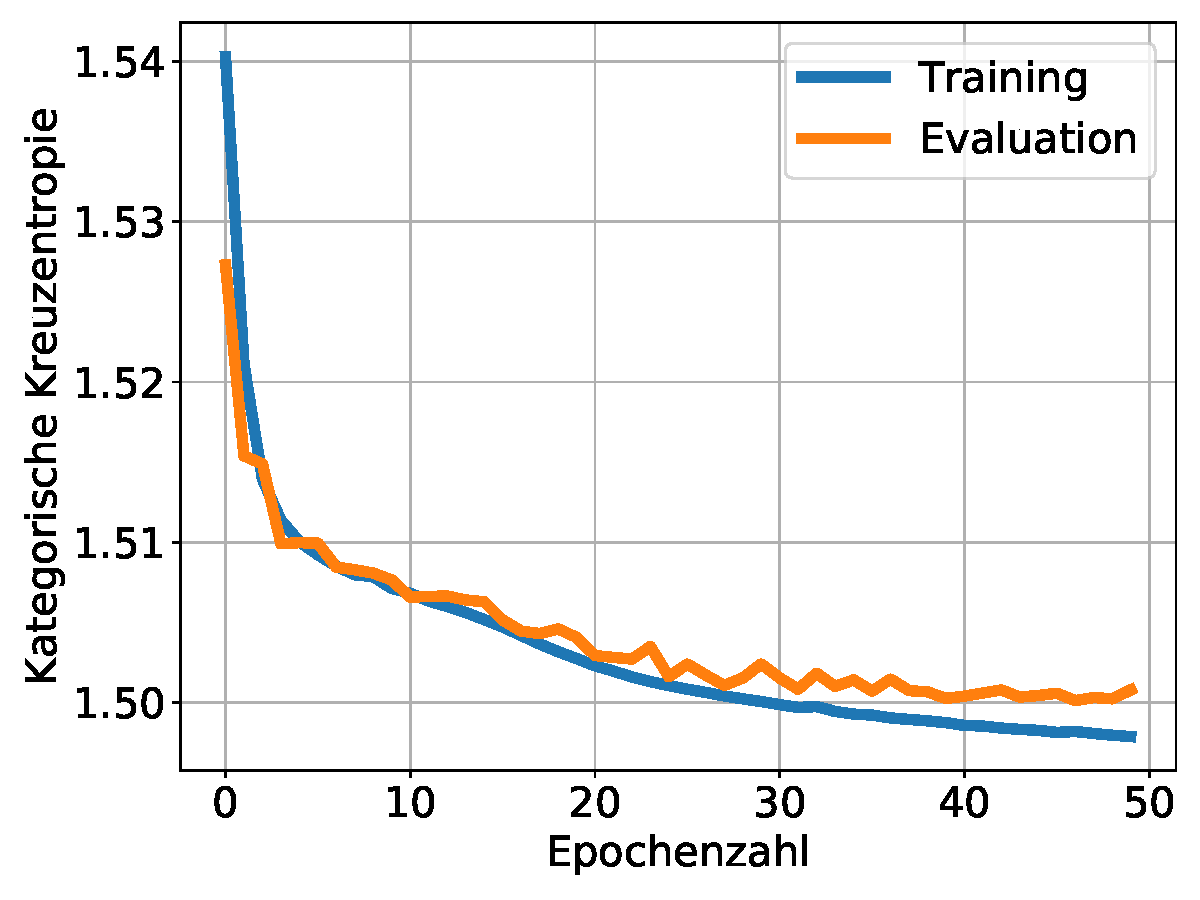
\includegraphics[height=5cm]{Plots/NN/loss.pdf}%
        \caption{Kostenfunktion: Kategorische Kreuzentropie}%
        \label{fig:NN_loss}%
    \end{subfigure}%
    \hfill% Fills available space in the center -> space between figures
    \begin{subfigure}{0.5\textwidth}%
        \centering%
        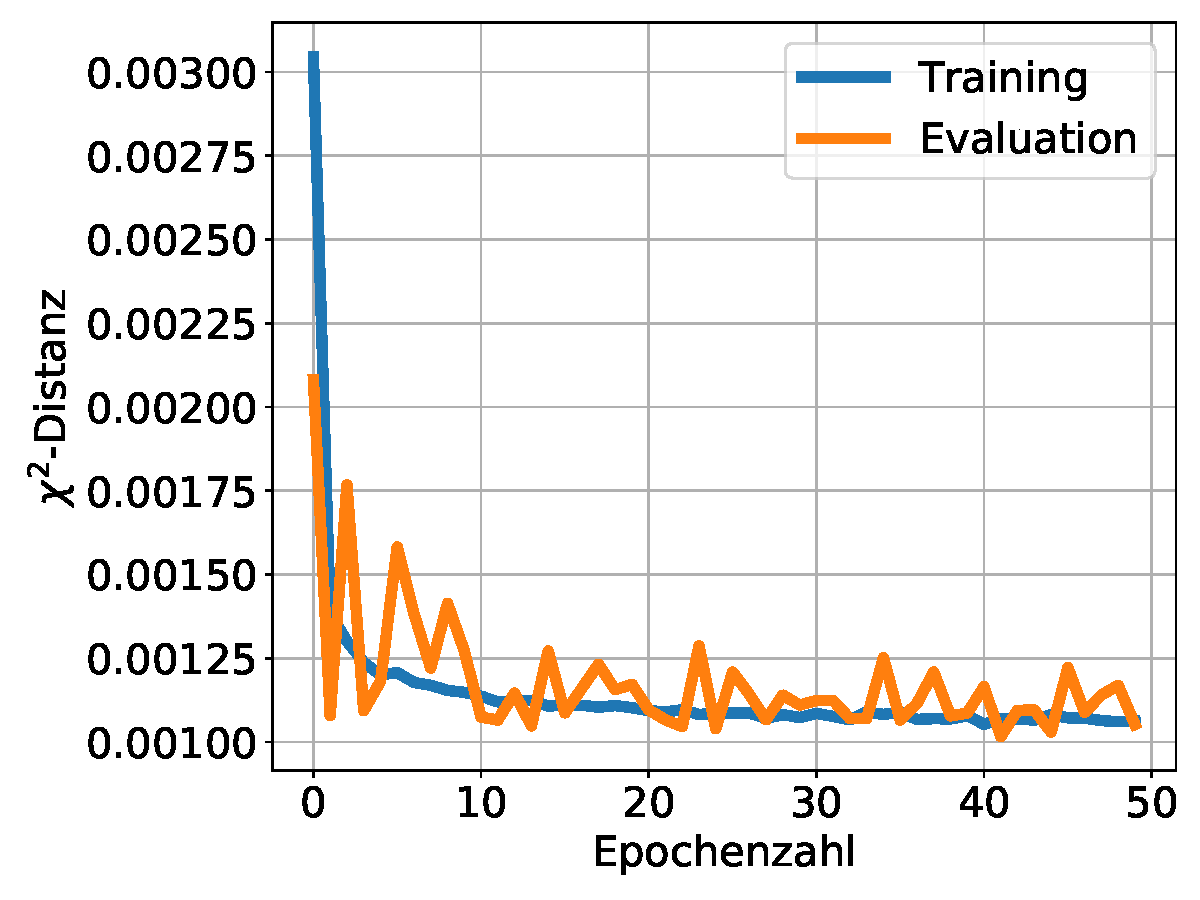
\includegraphics[height=5cm]{Plots/NN/chi.pdf}%
        \caption{Metrik: $\Chi^2$-Distanz}%
        \label{fig:NN_chi}%
    \end{subfigure}%
    \caption[Verlauf des Trainingsprozesses des NN ohne DSEA]{Verlauf des Trainingsprozess des NN.
    Zum einen ist die Kostenfunktion \textit{kategorische Kreuzentropie} und zum anderen die \textit{Chi-Quadrat-Distanz} als Metrik in Abhängigkeit der Epochenzahl aufgeführt.
    }
    \label{fig:NN_history}%
\end{figure}%

\begin{figure}
    \centering
    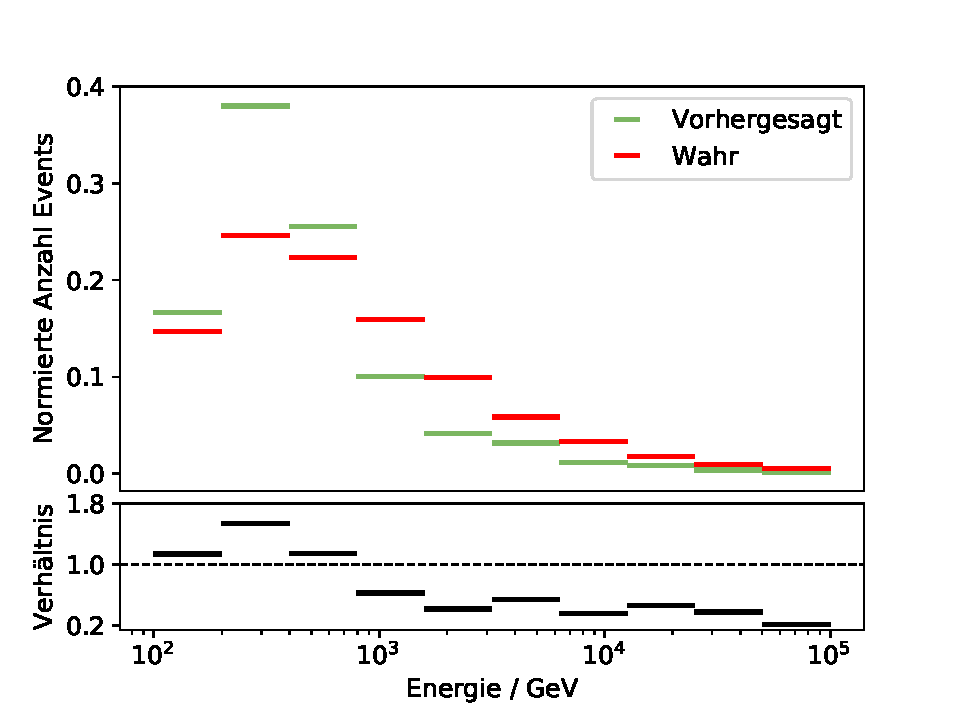
\includegraphics[width=\textwidth]{Plots/NN/spectrum_hard_10bins_50ep_500000samples_200pulls.pdf}
    \caption[Spektrum des NN ohne DSEA bei einer Klassifikation nach dem "`maximum a posterioro"'-Prinzip]{Das vorhergesagte und wahre Spektrum für ein NN, wenn ein Event der maximal vorhergesagten Klasse zugeordnet wird.
    Der untere Teil zeigt das Verhältnis zwischen wahrem und vorhergesagtem Spektrum und ist ein Maß für die relative Abweichung.
    Energien bis etwa \SI{1}{\tera\electronvolt} werden systematisch überschätzt, wobei die hochenergetischen Events unterschätzt werden.
    }
    \label{fig:NN_spectrum_hard}
\end{figure}
Die zweite grundlegende Idee die DSEA definiert, ist die \textbf{Wahrscheinlichkeitsinterpretation} der Konfidenzen $c_{ij}$.
Anstatt die Klasse mit der größten Konfidenz zu wählen, werden die Konfidenzen für jede Zielklasse aufsummiert (\autoref{eq:dsea_confidence}).
Die \autoref{fig:NN_spectrum} zeigt das resultierende Spektrum mit zugehöriger Abweichung.
\begin{figure}
    \centering
    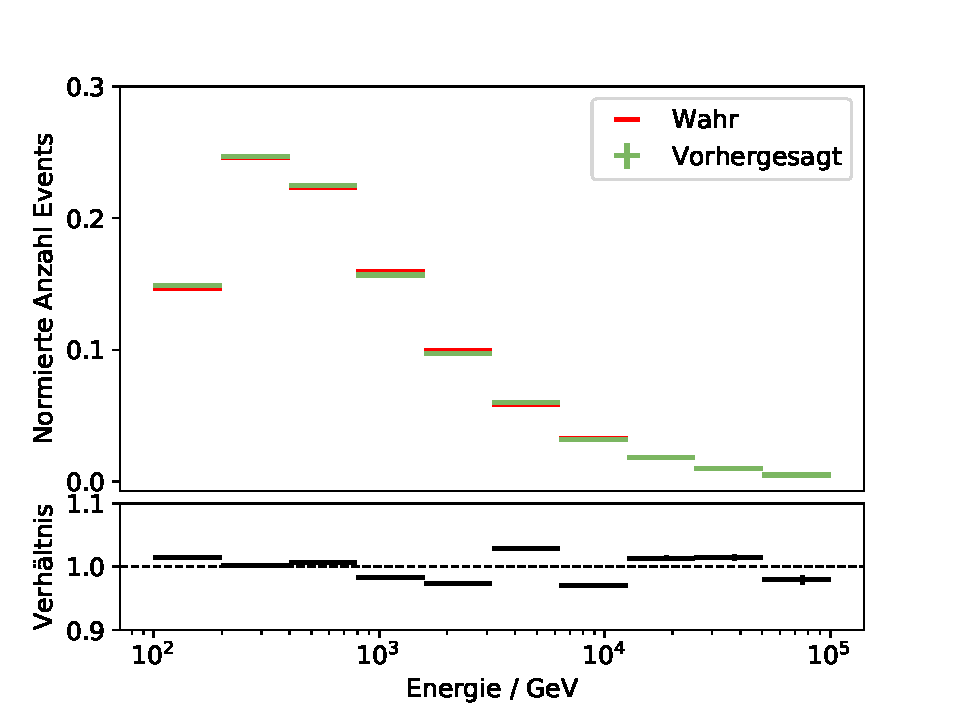
\includegraphics[width=0.9\textwidth]{Plots/NN/spectrum_dist_10bins_50ep_500000samples_200pulls.pdf}
    \caption[Spektrum des NN ohne DSEA mit Beachtung der Wahrscheinlichkeitsinterpretation]{Vorhergesagtes und wahres Spektrum für ein NN, wenn die Konfidenzen für jeden Bin aufsummiert werden.
    Der untere Teil zeigt das Verhältnis zwischen wahrem und vorhergesagtem Spektrum und dient als Maß für die relative Abweichung.
    Bestimmung der Unsicherheiten über das Bootstrapping-Verfahren, siehe \autoref{sec:bootstrap}.
    }
    \label{fig:NN_spectrum}
\end{figure}
Die Vorhersage stimmt hier weitgehend mit dem wahren Spektrum überein, wie auch der Verhältnis-Plot zeigt.
Größere Abweichungen sind in den Hochenergie-Bins zu beobachten.
Dort treten auch die für eine Entfaltung typischen Oszillationen auf.
\\
\\
Wie die Vorhersage einzelner Events (\autoref{fig:NN_single_events}) andeutet, wird durch die in \autoref{fig:nn_correlation} dargestellte Korrelationsmatrix bestätigt.
Es gibt eine starke Korrelation zwischen benachbarten Bins.
Grund dafür ist die ordinale Natur des Problems.
Jede Klasse repräsentiert bestimmte Energien, die einer definierten Ordnung folgen.
\begin{figure}
    \centering
    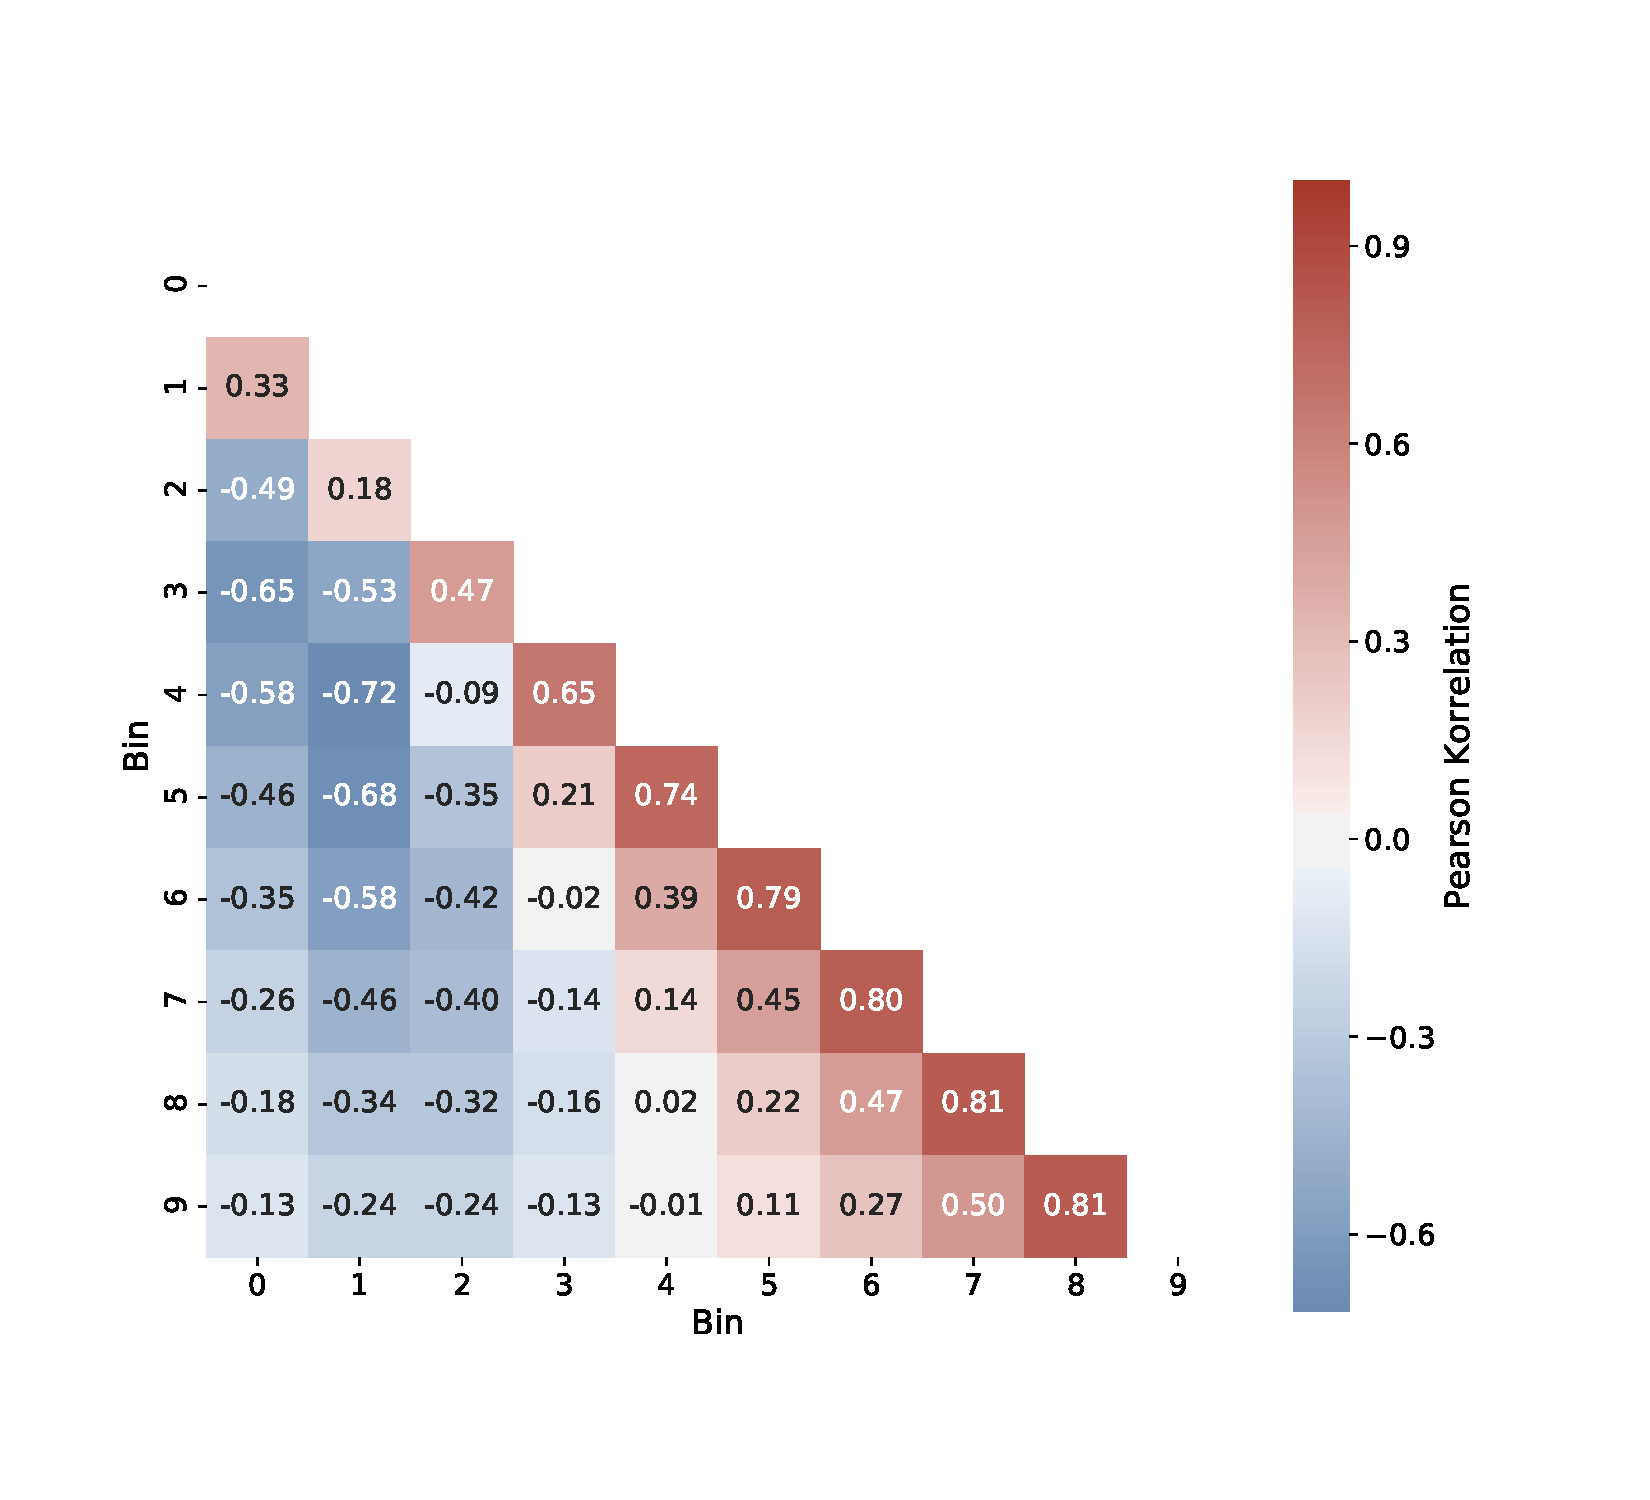
\includegraphics[width=\textwidth]{Plots/NN/correlation_matrix.pdf}
    \caption[Korrelationsmatrix des NN ohne DSEA]{Darstellung der relevanten Komponenten der symmetrischen Korrelationsmatrix.
    Sie gibt die Korrelationen zwischen den \SI{10}{\text{Bins}} für das NN an.
    }
    \label{fig:nn_correlation}
\end{figure}

% NN IN DSEA
\section{Entfaltung mit DSEA} \label{sec:deconv_dsea}
\subsection{Initialisierung}
DSEA ist für Klassifikationsalgorithmen der Scikit-Learn-Bibliothek\cite{scikit-learn} ausgerichtet.
Diese ist nicht für die Implementierung neuronaler Netze optimiert.
In der Arbeit wird dazu das Framework \textit{Tensorflow}\cite{tensorflow2015-whitepaper} und dessen API \textit{Keras} verwendet.
\\
Statt den Quellcode von DSEA anzupassen, wird ein Wrapper ("Verpackung") für die Keras-API entwickelt.
Der Wrapper kann im Anhang \ref{code:wrapper} eingesehen werden.
\\
Die Methoden \textit{fit()} und \textit{predict()} sind, wie die Methoden der Klassifizierer der Scikit-Learn-Bibliothek aufgebaut.
Die Konsequenz ist, dass bereits bei der Initialisierung die Hyperparameter übergeben werden.
Das sind Parameter die üblicherweise in der \textit{fit()} Methode auftreten. 
Betroffen sind die Anzahl der Epochen, Batchgröße und die Lernrate.
\\
Der neu eingeführte Parameter \textbf{one\_model} $[$Bool$]$ gibt an, ob im gesamten Trainingsprozess nur ein Modell verwendet wird:

\begin{description}
    \item [True]Ein Modell wird trainiert, wobei die Gewichte in jeder DSEA-Iteration aktualisiert werden
    \item [False]In jeder DSEA-Iteration wird ein neues Modell erstellt, welches auf den angepassten Gewichten trainiert wird
\end{description}
Die meisten Klassifizierer basieren nicht auf einer Verlustfunktion und können somit den Trainingsprozess nicht fortsetzen.
Das bedeutet, dass die Klassifizierer der Scikit-Learn-Bibliothek in jeder DSEA-Iteration neu initialisiert werden.
NN in DSEA bieten also die Freiheit, zwischen den beiden Szenarien zu wählen.
\\
Die Anzahl an Epochen pro DSEA \textit{Iteration} ist durch den Parameter \textit{Epochen} definiert.
Die Gesamtanzahl der Epochen ergibt sich durch \textit{Epochen} $\times$ \textit{Iterationen}.

% Gridsearch
\subsection{Optimierung der Hyperparameter}
Zur systematischen Untersuchung der drei Parameter \textit{Anzahl Epochen}, \textit{Anzahl Iterationen in DSEA} und \textit{one\_model} wird eine Gittersuche durchgeführt.
Es wird das bereits bekannte Modell \ref{tab:nn_shape} mit der gleichen Batchsize und Lernrate verwendet.
Aufgrund der Rechenzeit wird für die Gittersuche nur ein Teil des Trainingsdatensatzes mit $\sim \SI{1000000}{\text{Events}}$ genutzt.
\\
Zur Evaluation der Modelle werden die Abstände zwischen dem wahren und entfalteten Spektrum betrachtet.
Es werden $\sim \SI{500000}{\text{Events}}$ entfaltet und ausgewertet.
In \autoref{tab:gridsearch} sind die Parameter der 10 besten Modelle der Gittersuche, nach der $\Chi^2$-Distanz sortiert, aufgelistet.

\begin{table}
    \centering
    \caption{Die 10 besten Modelle der Gittersuche für die Parameter \textit{Anzahl Epochen}, \textit{Anzahl Iterationen in DSEA} und \textit{one\_model} aufgeführt. Die Ergebnisse sind nach der $\Chi^2$-Distanz sortiert. Ebenfalls ist der Root Mean Square Error (RMSE) angegeben.}
    \label{tab:gridsearch}
    \begin{tabular}{l l l | l l}
        \toprule
        Epochen & Iterationen &	one\_model & RMSE & $\Chi^2$-Distanz \\
        \midrule
        \rowcolor{tugreen}
        $75	$ & $12$ & False & $0.003123$ & $0.000269$ \\
        \rowcolor{tugreen}
        $60	$ & $16$ & True & $0.003282$ & $0.000293$ \\
        $50	$ & $16$ & True & $0.004092$ & $0.000439$ \\
        $50	$ & $8$ & False & $0.004332$ & $0.000449$ \\
        $10	$ & $12$ & True & $0.005303$ & $0.000518$ \\
        $100$ & $20$ & False & $0.006635$ & $0.000623$ \\
        $25	$ & $12$ & False & $0.006319$ & $0.000653$ \\
        $100$ & $16$ & True & $0.006286$ & $0.000686$ \\
        $25	$ & $16$ & True & $0.005821$ & $0.000688$ \\
        $75	$ & $8$ & True & $0.005655$ & $0.000694$ \\
        \bottomrule
    \end{tabular}
\end{table}
Ebenfalls wird der Root Mean Square Error (\glqq Wurzel des mittleren quadratischen Fehlers\grqq), kurz \textbf{RMSE} als Abstandsmaß betrachtet.
\\
Zur Veranschaulichung sind die Ergebnisse in einem Streudiagramm für \textit{one\_model=True} in \autoref{fig:scatter_true} bzw. für \textit{one\_model=False} in \autoref{fig:scatter_false} dargestellt.
Die logarithmisch skalierte Farbskala gibt die $\Chi^2$-Distanz an.
Auffällig ist, dass bei einer geringen Anzahl an Iterationen in DSEA der Abstand besonders groß ist.
Mit steigender Anzahl an Iterationen konvergiert dieser.
\\
Im Bezug auf die Anzahl der Epochen liegen die Modelle mit den kleinsten Abständen zwischen 50 und \SI{75}{\text{Epochen}}.
\\
Die zwei Modelle mit dem geringsten $\Chi^2$-Abstand werden genauer untersucht:

\begin{minipage}{0.44\textwidth}
    %\centering
    {\color{tugreen} \underline{\textbf{Modell 1}}}
    \begin{description}
        \item [Epochenzahl] 75
        \item [Iterationen] 12
        \item [one\_model] False
        \item [Grafiken] im Anhang \ref{fig:dsea_history_false} \ref{fig:dsea_spectrum_false} \ref{fig:dsea_correlation_false}
    \end{description}
\end{minipage}%
\vline
\hfill
\begin{minipage}{0.48\textwidth}
    %\centering
    {\color{tugreen} \underline{\textbf{Modell 2}}}
    \begin{description}
        \item [Epochenzahl] 60
        \item [Iterationen] 16
        \item [one\_model] True
        \item [Grafiken] in Abbildung \ref{fig:dsea_history_true} \ref{fig:dsea_spectrum_true} \ref{fig:dsea_correlation_true}
    \end{description}
\end{minipage}%

In den folgenden Abschnitten \ref{sec:dsea_training} bis \ref{sec:dsea_correlation} wird exemplarisch die Trainingshistorie, das Energiespektrum und die Korrelationsmatrix des 2. Modells gezeigt.
Analog dazu befinden sich die Plots des 1. Modells der Übersichtlichkeit halber im Anhang.
\begin{figure}
    \centering
    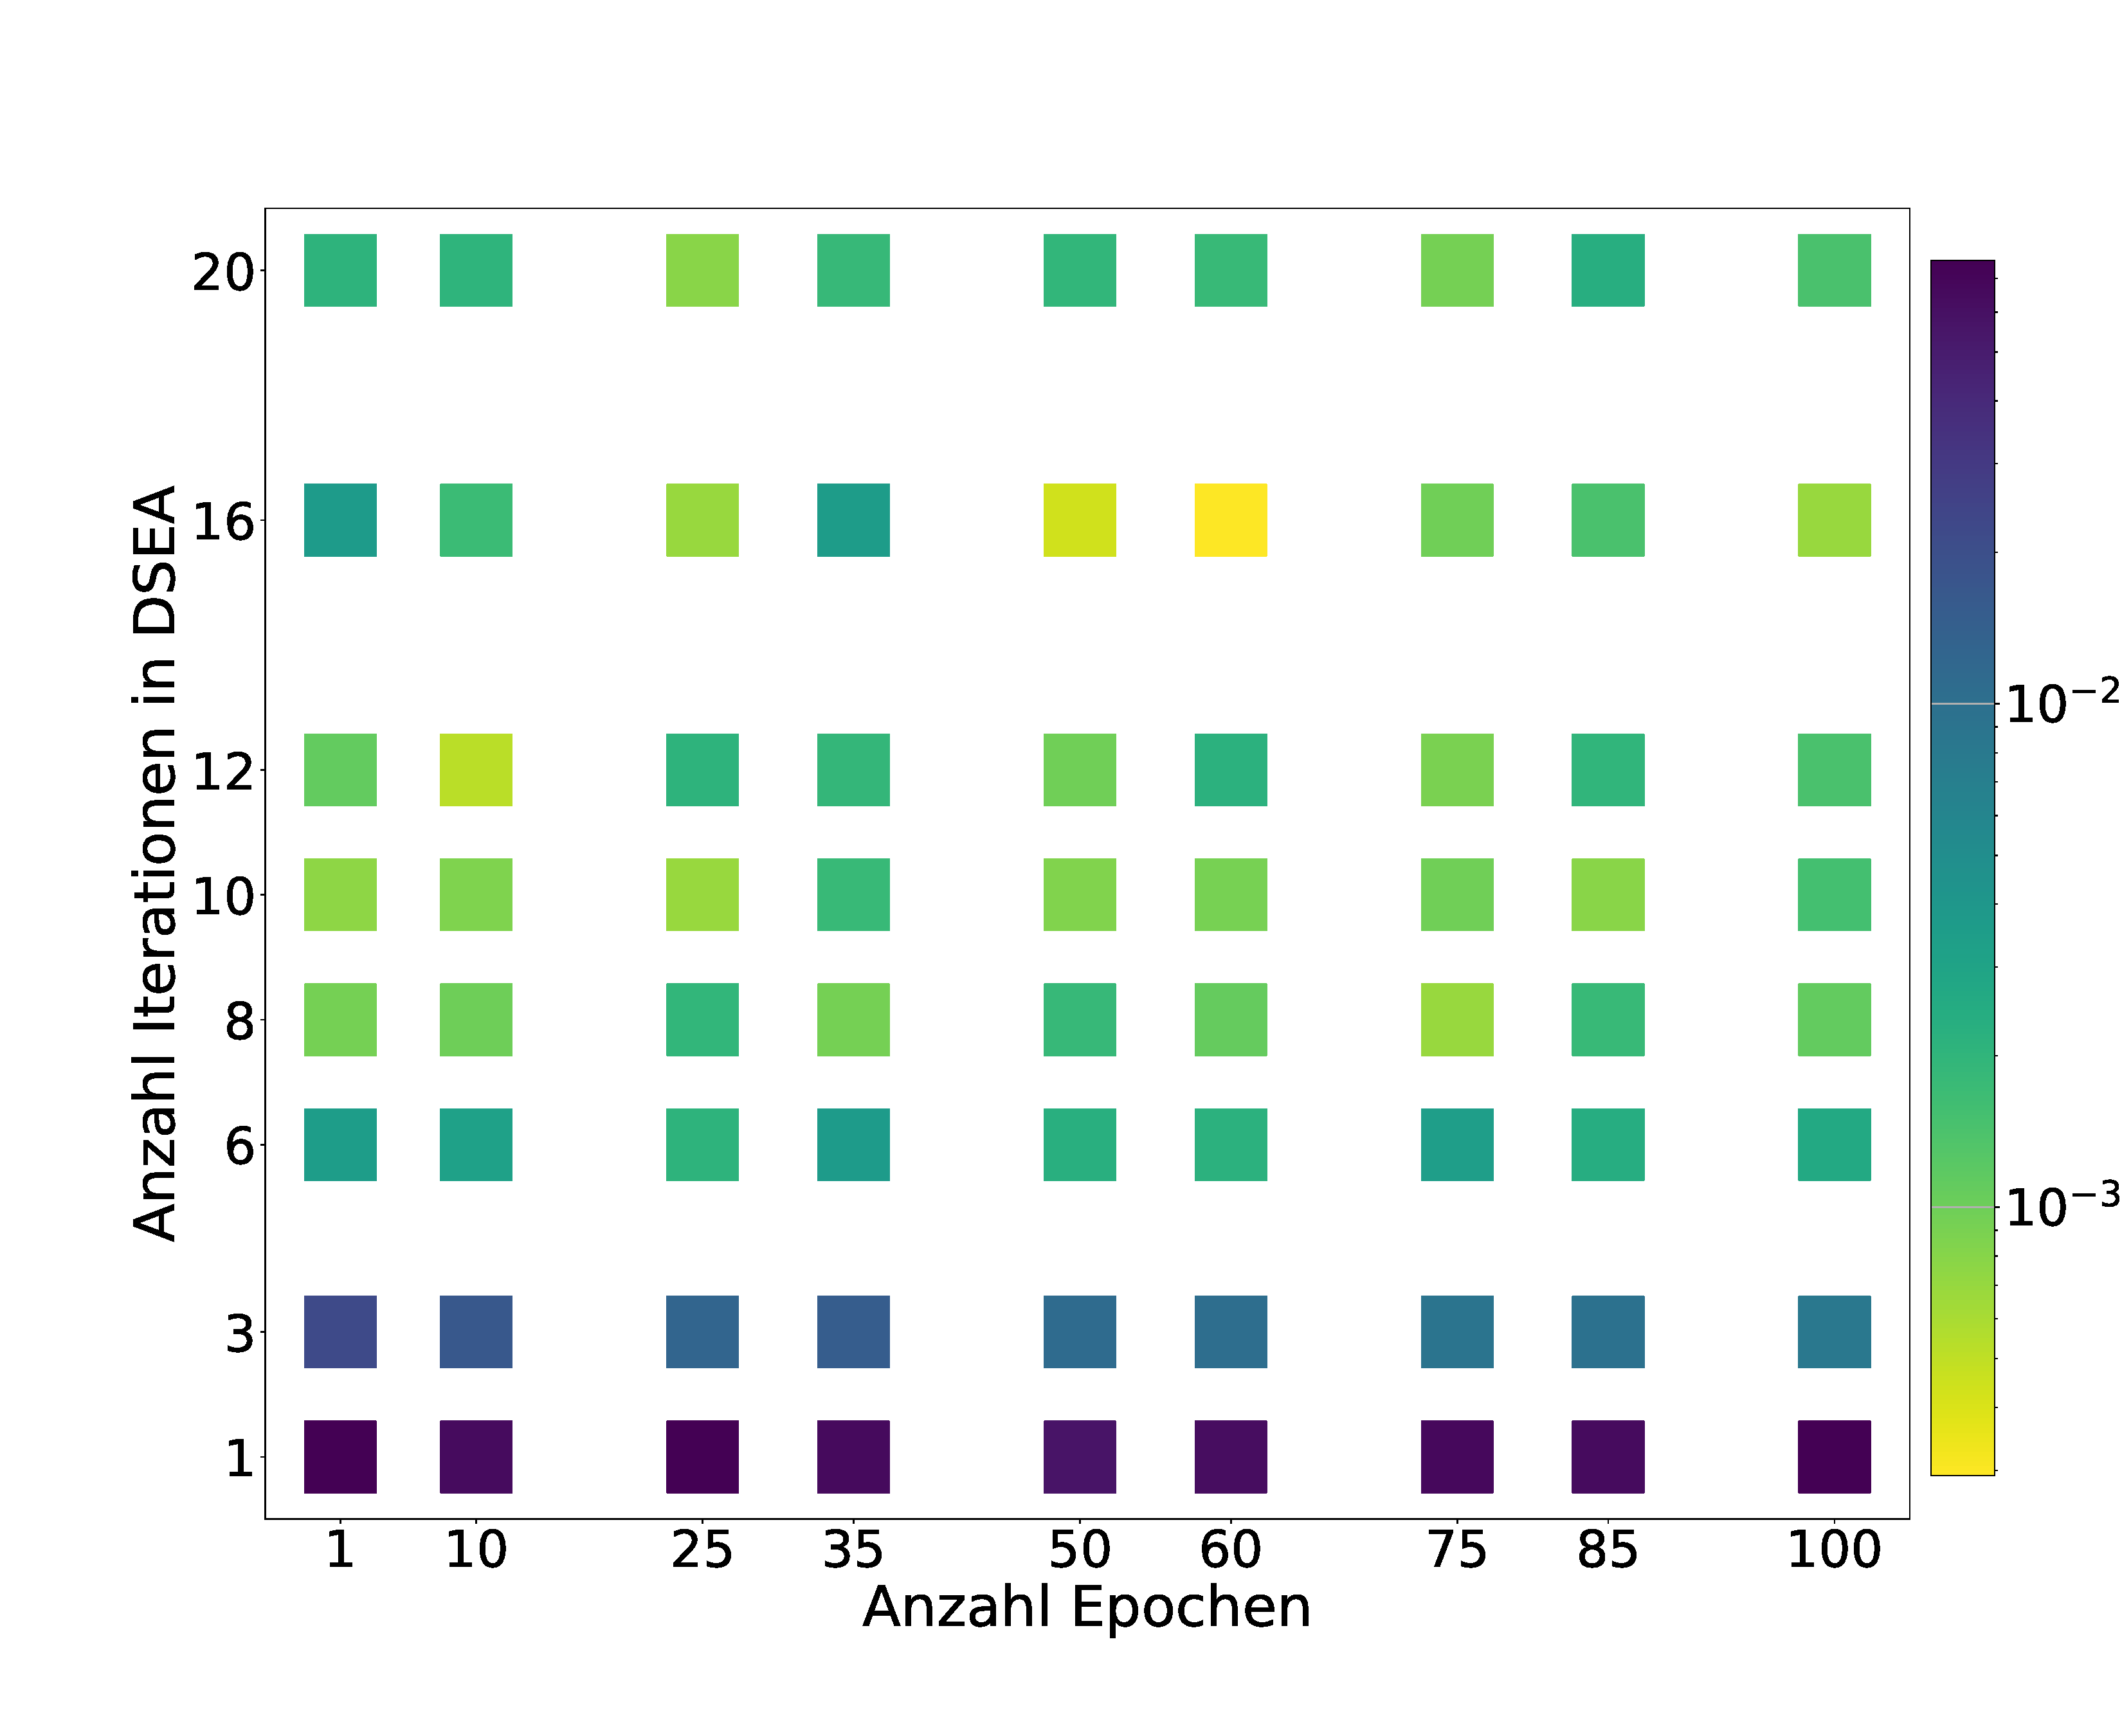
\includegraphics[width=\textwidth]{Plots/DSEA/True/scatter_chi2.pdf}
    \caption[Ergebnisse der Gittersuche für ein NN in DSEA]{Streudiagramm zur Darstellung der Ergebnisse der Gittersuche für \textit{one\_model=True}.
    Der Trainingsprozess des Modells wird in jeder DSEA-Iteration mit angepassten Gewichten fortgesetzt.
    Die logarithmisch-skalierte Farbskala gibt den $\Chi^2$-Abstand zwischen dem wahren und vorhergesagten Spektrum an.
    }
    \label{fig:scatter_true}
\end{figure}

% Trainingsprozess
\subsection{Trainingsprozess} \label{sec:dsea_training}
Der Verlauf des Trainingsprozess des 2. Modells in \autoref{fig:dsea_history_true} hat einen näherungsweisen stetigen Verlauf.
\begin{figure}%
    \begin{subfigure}{0.5\textwidth}%
        \centering%
        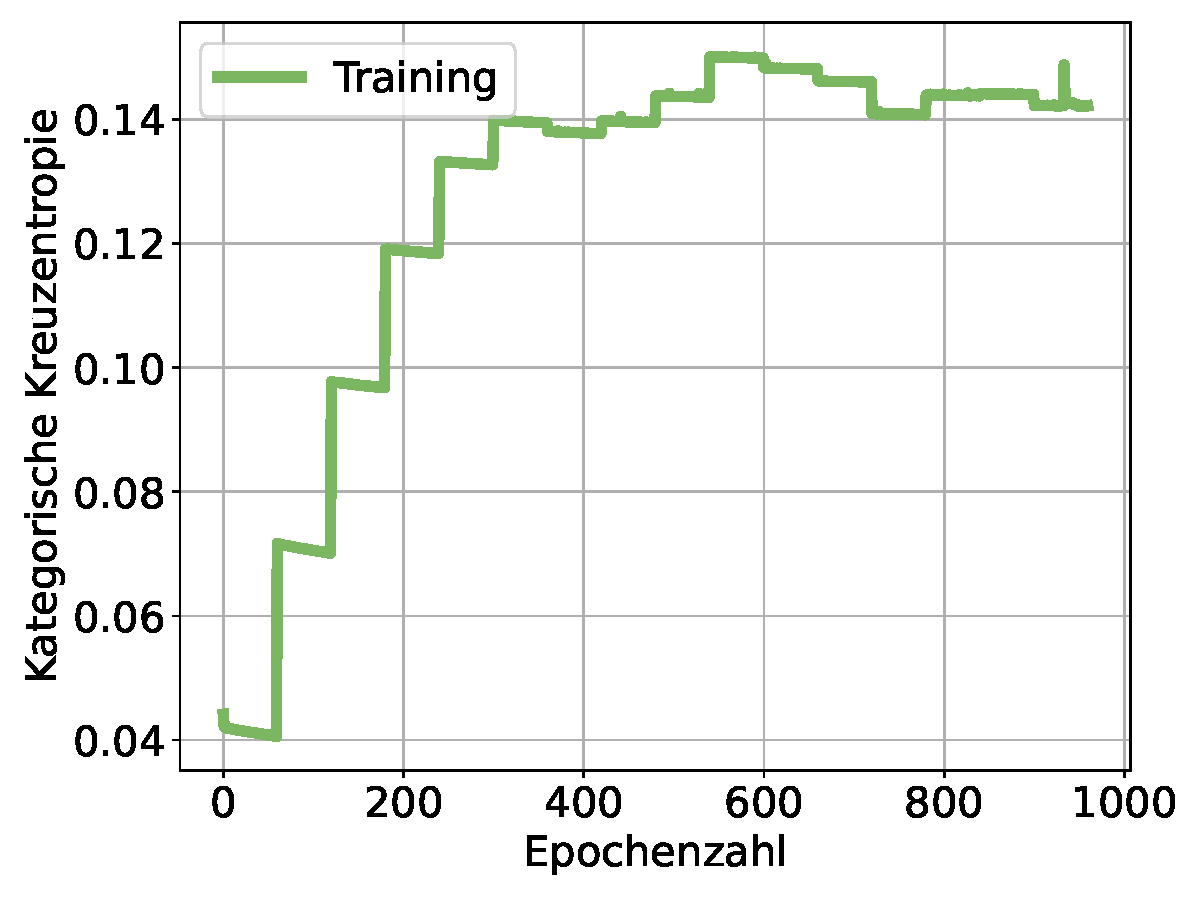
\includegraphics[height=5cm]{Plots/DSEA/True/loss.pdf}%
        \caption{Kostenfunktion: Kategorische Kreuzentropie}%
        %\label{fig:NN_loss}%
    \end{subfigure}%
    \hfill% Fills available space in the center -> space between figures
    \begin{subfigure}{0.5\textwidth}%
        \centering%
        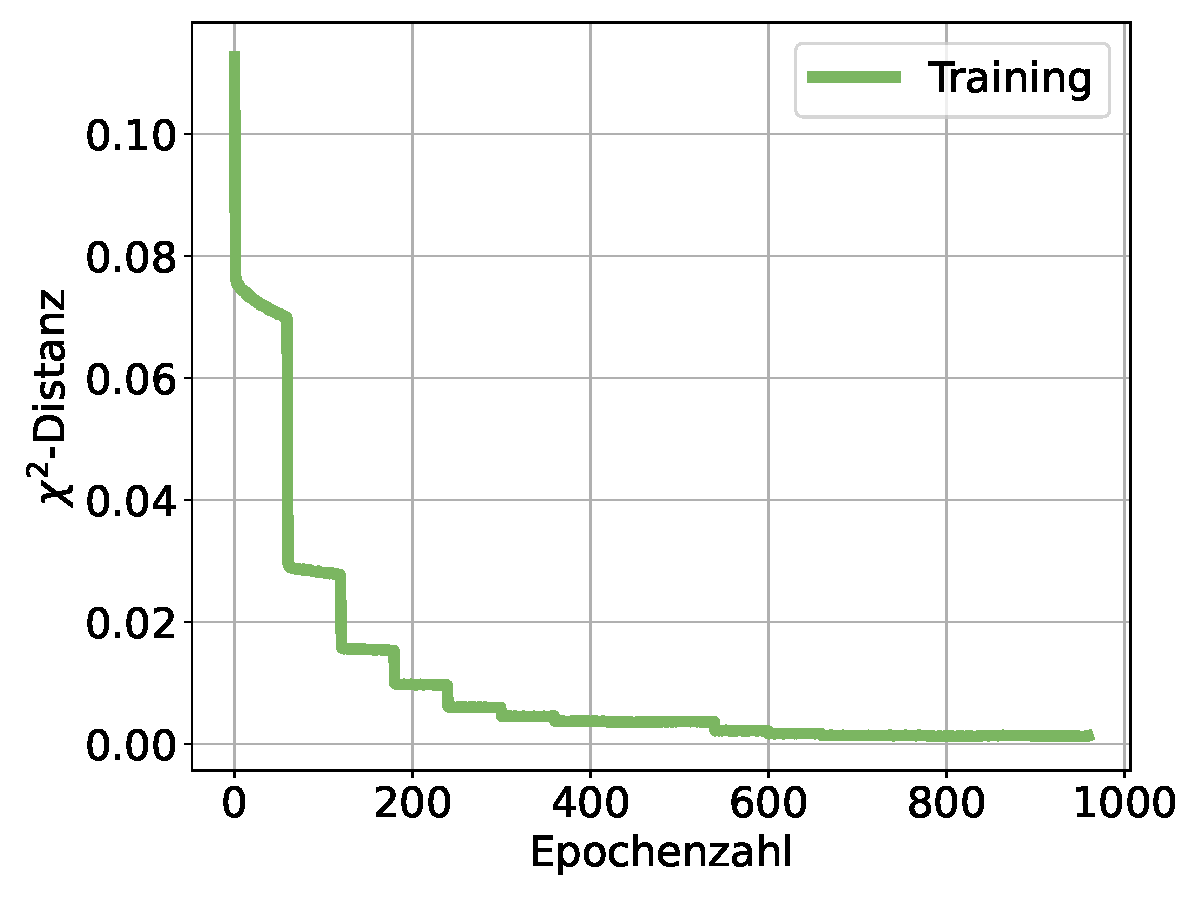
\includegraphics[height=5cm]{Plots/DSEA/True/chi.pdf}%
        \caption{Metrik: $\Chi^2$-Distanz}%
        %\label{fig:NN_chi}%
    \end{subfigure}%
    \caption[Verlauf des Trainingsprozess des 2. Modells in DSEA]{Verlauf des Trainingsprozess des 2. Modells mit dem Parameter \textit{one\_model=True}.
    Im gesamten Trainingsverlauf wird ein Modell trainiert, wobei die Gewichte in jeder DSEA-Iteration angepasst werden.
    Zum einen ist die Kostenfunktion \textit{kategorische Kreuzentropie} und zum anderen die \textit{Chi-Quadrat-Distanz} als Metrik in Abhängigkeit der Epochenzahl aufgeführt.
    }
    \label{fig:dsea_history_true}%
\end{figure}%}
Das liegt daran, dass über den gesamten Prozess nur die Kostenfunktion eines Modells betrachtet wird.
Kleine Unstetigkeiten werden durch die angepassten Gewichte am Ende jeder DSEA-Iteration verursacht.
\\
Anders sieht es bei dem Trainingsverlauf des 1. Modells in \autoref{fig:dsea_history_false} aus.
In jeder DSEA-Iteration wird ein neues Modell erstellt und die Optimierung der Kostenfunktion beginnt von vorne.
Dies ist der Grund für den sprungartigen Verlauf der Metrik und der Verlustfunktion.
\\
Die $\Chi^2$-Distanz beider Modelle sinkt mit der Epochenzahl und konvergiert.
Hingegen steigt die kategorische Kreuzentropie bei jeder Neugewichtung.
Die Gewichte werden in der Kostenfunktion aktualisiert und führen zu einem Anstieg.
Die angepasste Kostenfunktion wird in den darauffolgenden Epochen bis zur nächsten Iteration minimiert.
Sie konvergiert, wenn auch die Gewichte konvergieren.

% Spektrum (Bootstrap in Anhang)
\subsection{Spektrum} \label{sec:dsea_spectrum}
Das entfaltete Spektrum ist für das 2. Modell in \autoref{fig:dsea_spectrum_true} bzw. für das 1. Modell in \autoref{fig:dsea_spectrum_false} abgebildet.
Es treten Oszillationen im gesamten Energiebereich auf.
Diese verstärken sich, insbesondere bei Modell 1 zu höheren Energien.
\\
Auffällig sind auch die ungewöhnlich großen absoluten Abstände in den ersten vier Energie-Bins.
Aufgrund der hohen Statistik in diesen Bins (viele Events im niedrigen Energiebereich) werden hier kleine Abweichungen erwartet.
Eine mögliche Ursache ist, dass die Hochenergie-Bins eine stärkere Gewichtung als die Bins im niederenergetischen Bereich erfahren.
Dadurch werden die Events mit hohen Energien im Trainingsprozess mehr berücksichtigt.
Die Verteilung der Ergebnisse des Bootstrap-Verfahrens zur Bestimmung der Unsicherheiten kann im Anhang eingesehen werden (Modell 1 im Anhang \ref{fig:dsea_bootstrap_true}, Modell 2 im Anhang \ref{fig:dsea_bootstrap_false}).
\begin{figure}
    \centering
    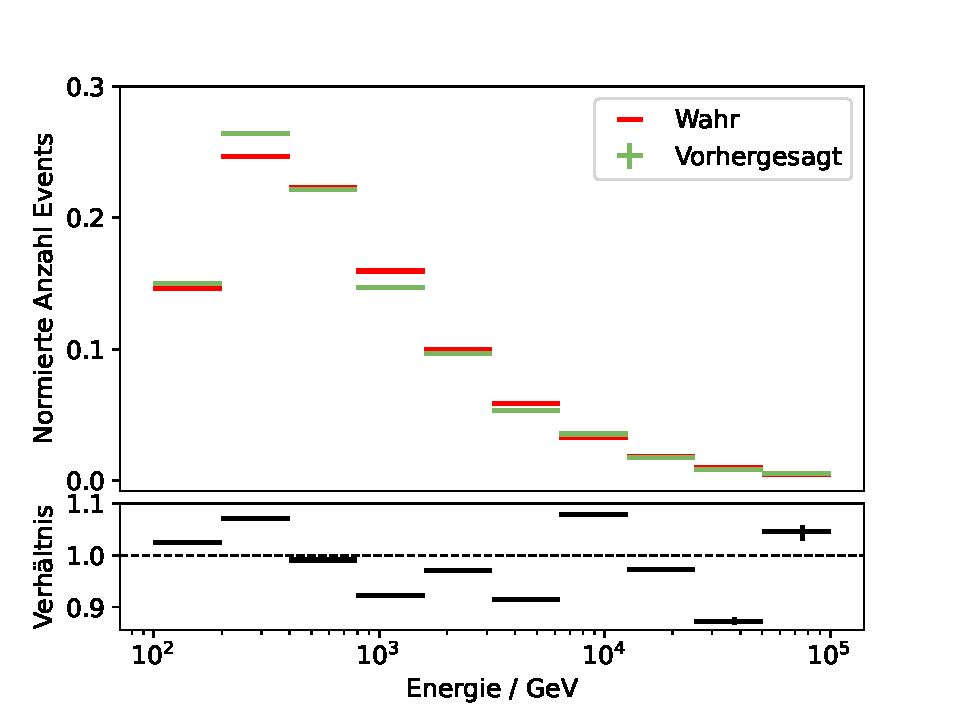
\includegraphics[width=0.9\textwidth]{Plots/DSEA/True/spectrum_dist_10bins_60ep_500000samples_200pulls.pdf}
    \caption[Spektrum des 2. Modells in DSEA]{Das entfaltete Spektrum des 2. Modells mit dem Parameter \textit{one\_model=True}.
    Im gesamten Trainingsverlauf wird ein Modell trainiert, wobei die Gewichte in jeder DSEA-Iteration angepasst werden.
    Der untere Teil zeigt das Verhältnis zwischen wahrem und vorhergesagtem Spektrum und dient als Maß für die relative Abweichung.
    }
    \label{fig:dsea_spectrum_true}
\end{figure}

% Correlation
\subsection{Korrelation} \label{sec:dsea_correlation}
Die Vorhersage einzelner Events (Modell 1 im Anhang \ref{fig:dsea_single_events_false}, Modell 2 im Anhang \ref{fig:dsea_single_events_true}) weisen für beide Modelle nur geringe Unterschiede auf.
Je nach Event variiert die Verteilung der Konfidenzen unterschiedlich stark.
\\
Aufällig sind hier die starken Korrelationen zu den benachbarten Bins.
Dies wird auch durch die Korrelationsmatrix in \autoref{fig:dsea_correlation_true} für Modell 2 (bzw. für Modell 1 im Anhang \ref{fig:dsea_correlation_false}) bestätigt.
\begin{figure}
    \centering
    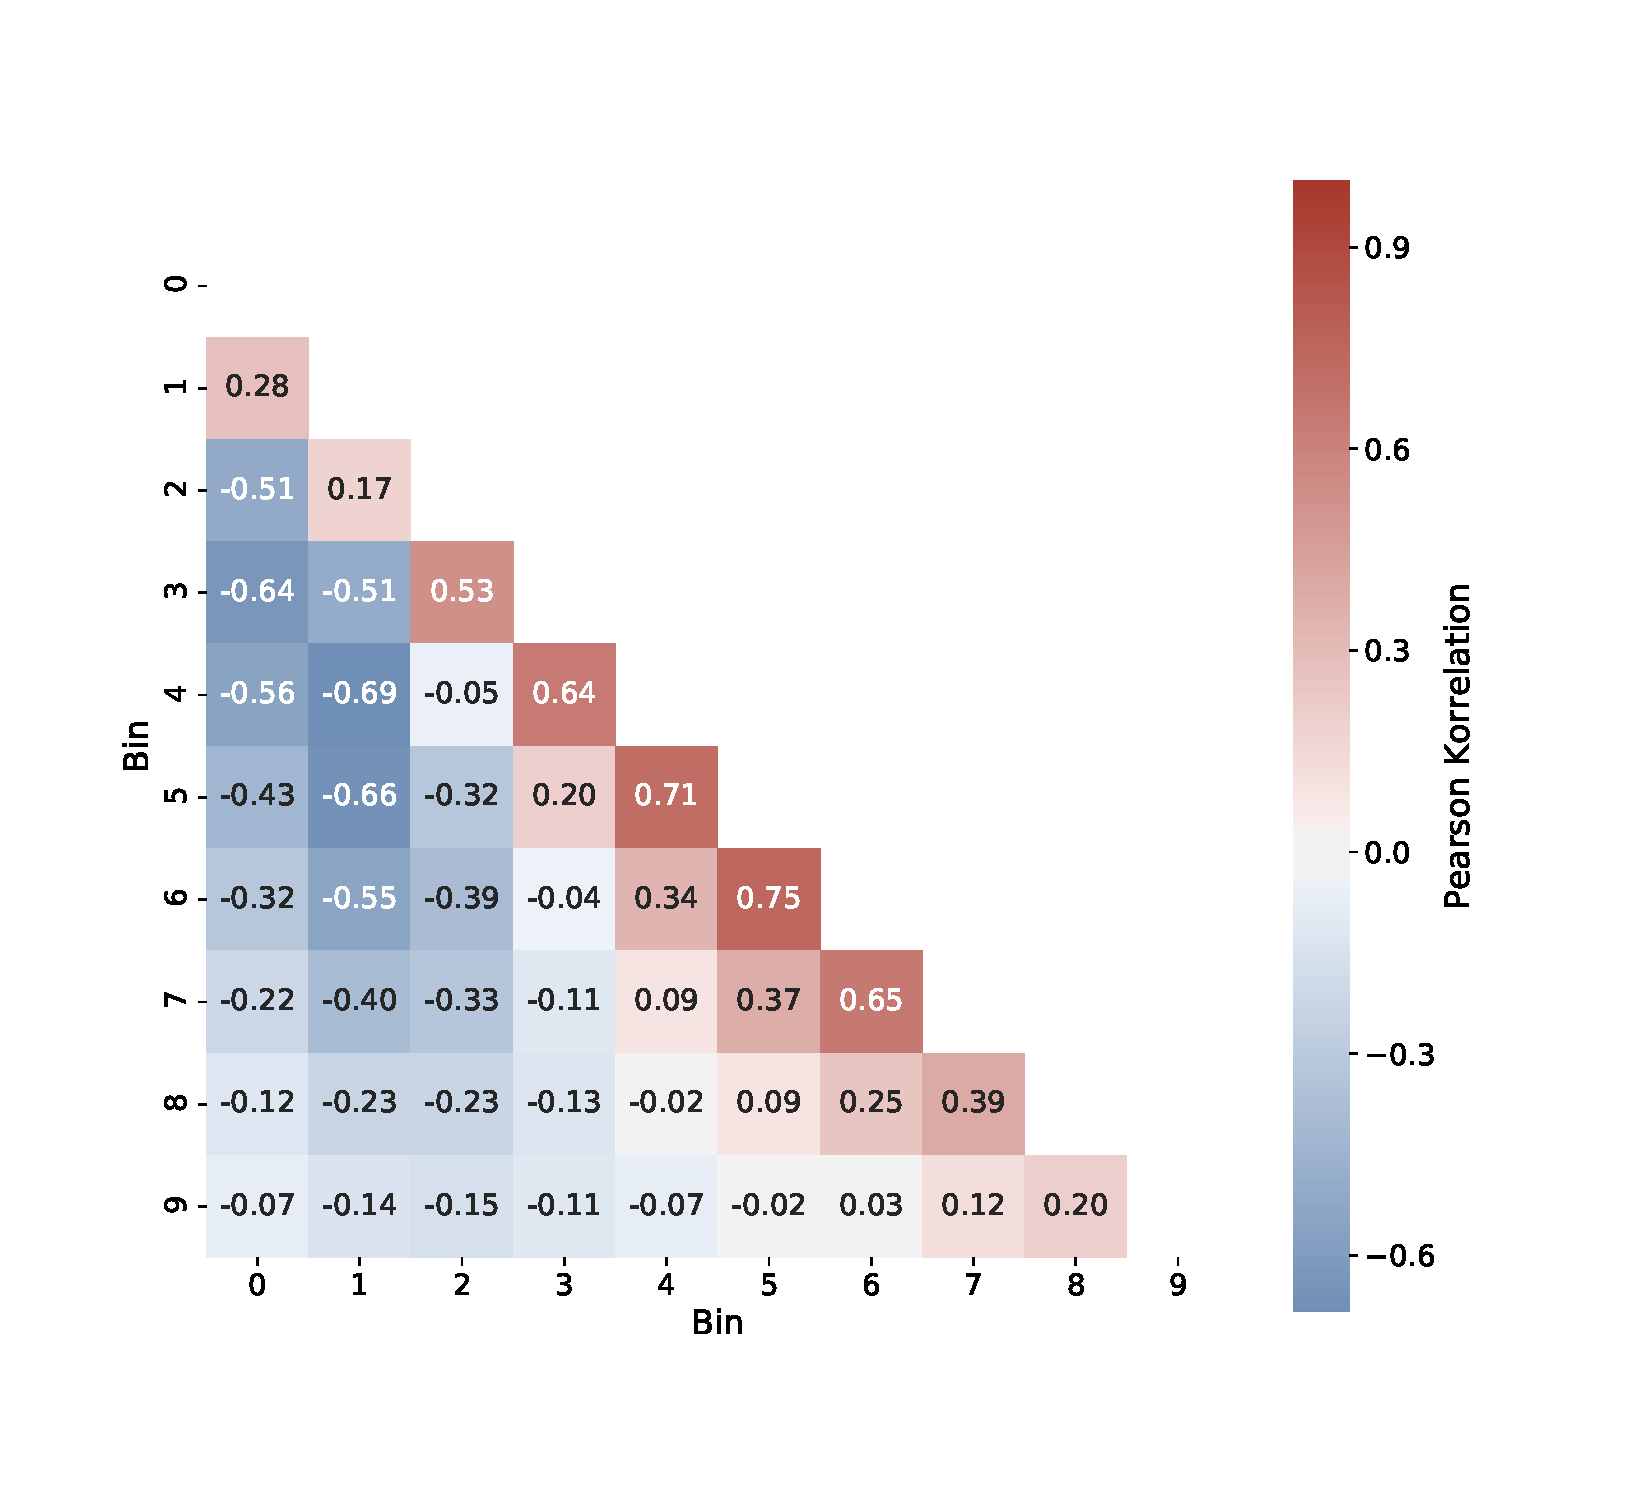
\includegraphics[width=1\textwidth]{Plots/DSEA/True/correlation_matrix.pdf}
    \caption[Korrelationsmatrix des 2. Modells in DSEA]{Die Korrelationsmatrix des 2. Modells (\textit{one\_model=True}).
    Sie gibt die Korrelationen zwischen den entfalteten Energie-Bins an.
    }
    \label{fig:dsea_correlation_true}
\end{figure}
Die benachbarten Bins sind stark positiv korreliert.
Wird also der $n$-te Bin vorhergesagt, so werden dem ($n$-1)-ten und ($n$+1)-ten Bin ebenfalls hohe Konfidenzen zugeordnet.
Die Korrelation nimmt zu entfernten Energien ab.
\\
Im niederenergetischen Bereich treten starke negative Korrelationen auf.
Insbesondere sind die Bins 3-6 mit Bin 1 korreliert.
Dies lässt sich auf die hohe Statistik im Bin 1 zurückführen.
Diesem Energiebereich sind die meisten Events zuzuordnen.
Wird nun exemplarisch der 4. Bin vorhergesagt, so wird dem 1. Bin eine niedrigere Konfidenz als im Durchschnitt zugeordnet.
% BIAS
\section{Abhängigkeit der Entfaltung vom Trainingsspektrum} \label{sec:bias}
In diesem Kapitel wird die Abhängigkeit des entfalteten Spektrums von den Trainingsdaten (\textit{Bias}) untersucht.
Dazu wird aus dem bekannten MC-Datensatz eine Teilprobe mit gleichverteilten Klassen erstellt.
Die Methode wird als \textit{Undersampling} bezeichnet.
\\
Die Probe beinhaltet von jeder der 10 Energie-Klassen \SI{50000}{\text{Events}} und umfasst somit insgesamt \SI{500000}{\text{Events}}.
Diese Teilprobe wird als Trainingsdatensatz verwendet.
Entfaltet und evaluiert werden \SI{500000}{\text{Events}} des bekannten Neutrino-Spektrums.
\\
Zum einen wird der Bias des gleichen NN, wie in \autoref{sec:nn_no_dsea} untersucht.
Zum anderen wird die Entfaltung eines NN in DSEA auf eine Abhängigkeit geprüft.
%Die Parameter des 1. Modells (siehe \autoref{sec:deconv_dsea}) sollen dabei verwendet werden.
% NN
\\
In \autoref{fig:bias_nn} sind die Ergebnisse des auf \SI{50}{\text{Epochen}} trainierten NN dargestellt.
\begin{figure}
    \centering
    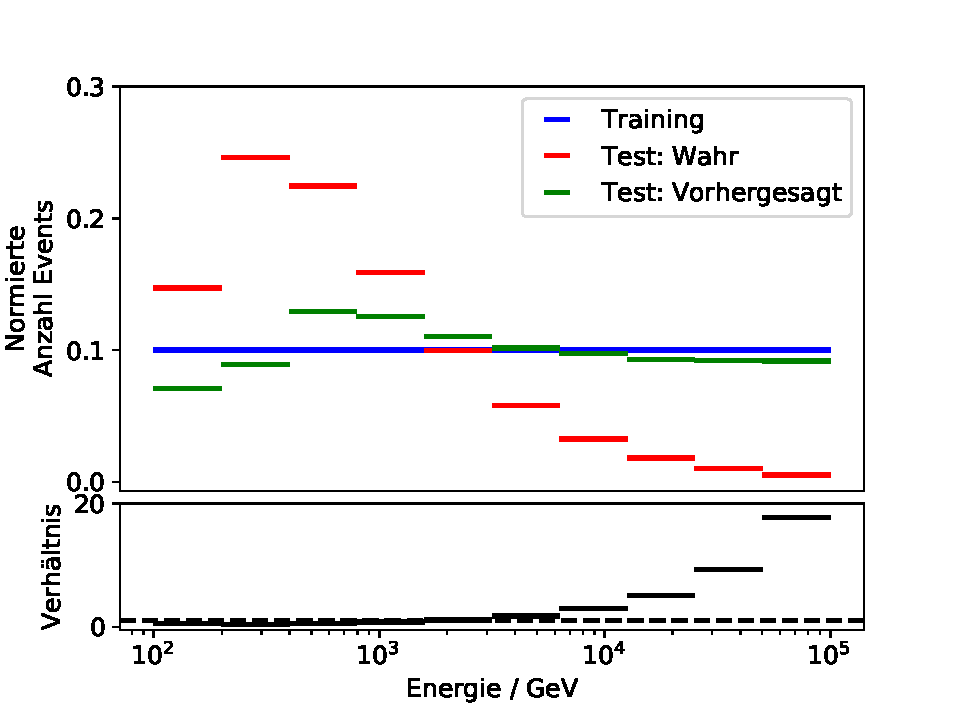
\includegraphics[width=0.9\textwidth]{Plots/BIAS/NN/spectrum.pdf}
    \caption[Überprüfung des Bias: Spektrum des NN ohne DSEA]{Das mit einem NN entfaltete Energiespektrum, der Neutrinos bei Verwendung von Trainingsdaten mit gleichverteilten Klassen.
    Vergleich der Spektren der Trainingsdaten (Blau), der wahren Evaluationsdaten (Rot) und der entfalteten Evaluationsdaten (Grün).
    }
    \label{fig:bias_nn}
\end{figure}
Zu sehen ist das Spektrum der gleichverteilten Trainingsdaten in Blau, der entfalteten Daten in Grün und des wahren Spektrums in Rot.
Das vorhergesagte Spektrum liegt nahe dem Trainingsspektrum.
Nur in Bin 3 und 4 wird das Maximum des zu entfaltenden Spektrums leicht angedeutet.
Insgesamt ist also ein starker Bias zu beobachten.
% DSEA
\\
Im folgenden wird das 1. Modell (\SI{12}{\text{Iterationen}}, \SI{75}{\text{Epochen}}, \textit{one\_model=False}) zur Entfaltung des Neutrino-Spektrums verwendet.
Trainiert wird das Modell auf den gleichverteilten Daten.
Die Spektren sind analog zum vorherigen Plot in \autoref{fig:bias_dsea_false} graphisch dargestellt.
Das entfaltete Spektrum unterscheidet sich erheblich von den Trainingsdaten.
Im Hochenergiebereich werden die Bins stark überschätzt.
Auch die anderen entfalteten Energiebereiche passen nur bedingt mit dem wahren Spektrum überein.
Dies liegt hier nicht an einer starken Abhängigkeit von den Daten, sondern lässt sich auf die geringe Accuracy zurückführen.
\\
Der gleiche Prozess wird für das 2. Modell (\SI{16}{\text{Iterationen}}, \SI{60}{\text{Epochen}}, \textit{one\_model=True}) durchgeführt.
Das entfaltete Spektrum in \autoref{fig:bias_dsea_true} weist starke Abweichungen von der wahren Verteilung auf.
Insbesondere die Hochenergie-Bins werden überschätzt.
Insgesamt unterscheiden sich die entfalteten Verteilungen signifikant von dem Trainingsspektrum.
Die Modellunabhängigkeit von DSEA wird dadurch wiedermal bestätigt.
\begin{figure}
    \centering
    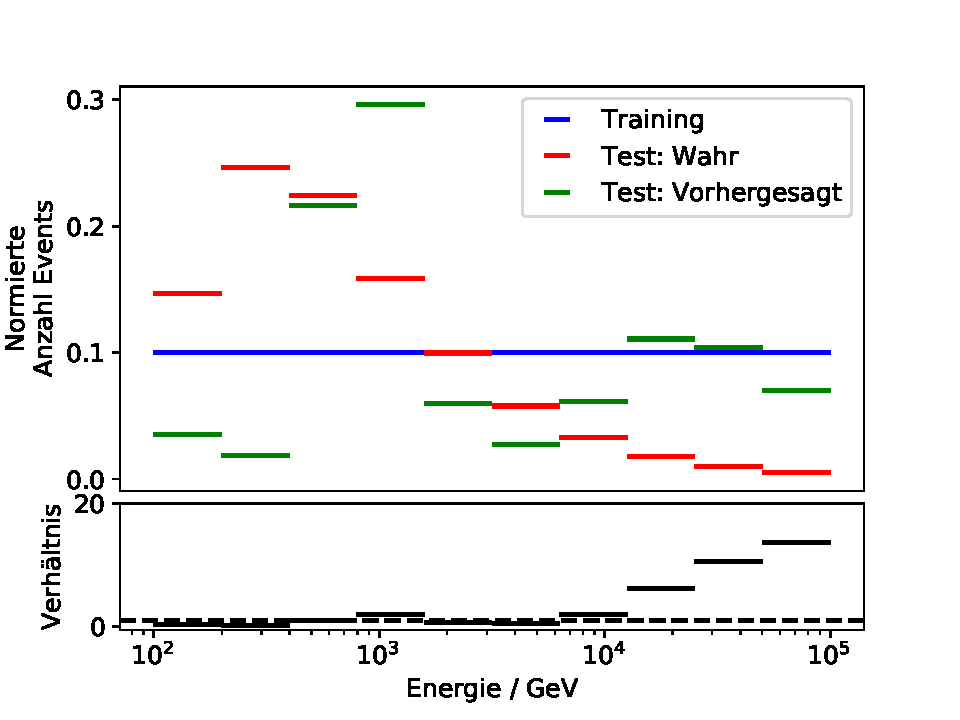
\includegraphics[width=0.9\textwidth]{Plots/BIAS/DSEA/spectrum_12it_75ep_False.pdf}
    \caption[Überprüfung des Bias: Spektrum des 1. Modells in DSEA]{Das mit einem NN in DSEA entfaltete Energiespektrum der Neutrinos.
    Das NN (Modell 1) wird in DSEA auf einem Datensatz mit gleichverteilten Klassen trainiert.
    Dargestellt ist das Spektrum der Trainingsdaten (Blau), der wahren Evaluationsdaten (Rot) und der entfalteten Evaluationsdaten (Grün).
    }
    \label{fig:bias_dsea_false}
\end{figure}
